\section{Modeling uncertainties}
\lb{sec:lowE_syst}

Include the models with different selection of low energies.
\subsection{Different low-energy ranges}
Our background template of the rectangles (baseline) and the low-energy model consists of source-class data averaged over the energy interval $0.3 - \SI{1.0}{GeV}$. To probe the dependence on the choice of the low-energy range of the rectangles model, we pick the three non-overlapping energy ranges $0.3 - \SI{0.5}{GeV}$, $0.5 - \SI{1.0}{GeV}$, and $1.0 - \SI{2.2}{GeV}$ and use the same analysis as for the baseline model. We also compare with the spectra of ultraclean-class data. The residual spectra resulting from the different energy ranges and data classes are shown in Figure \ref{fig:syst_models}. For high energies, with what this analysis is converned with, the agreement is very good. 
\begin{figure*}[h]
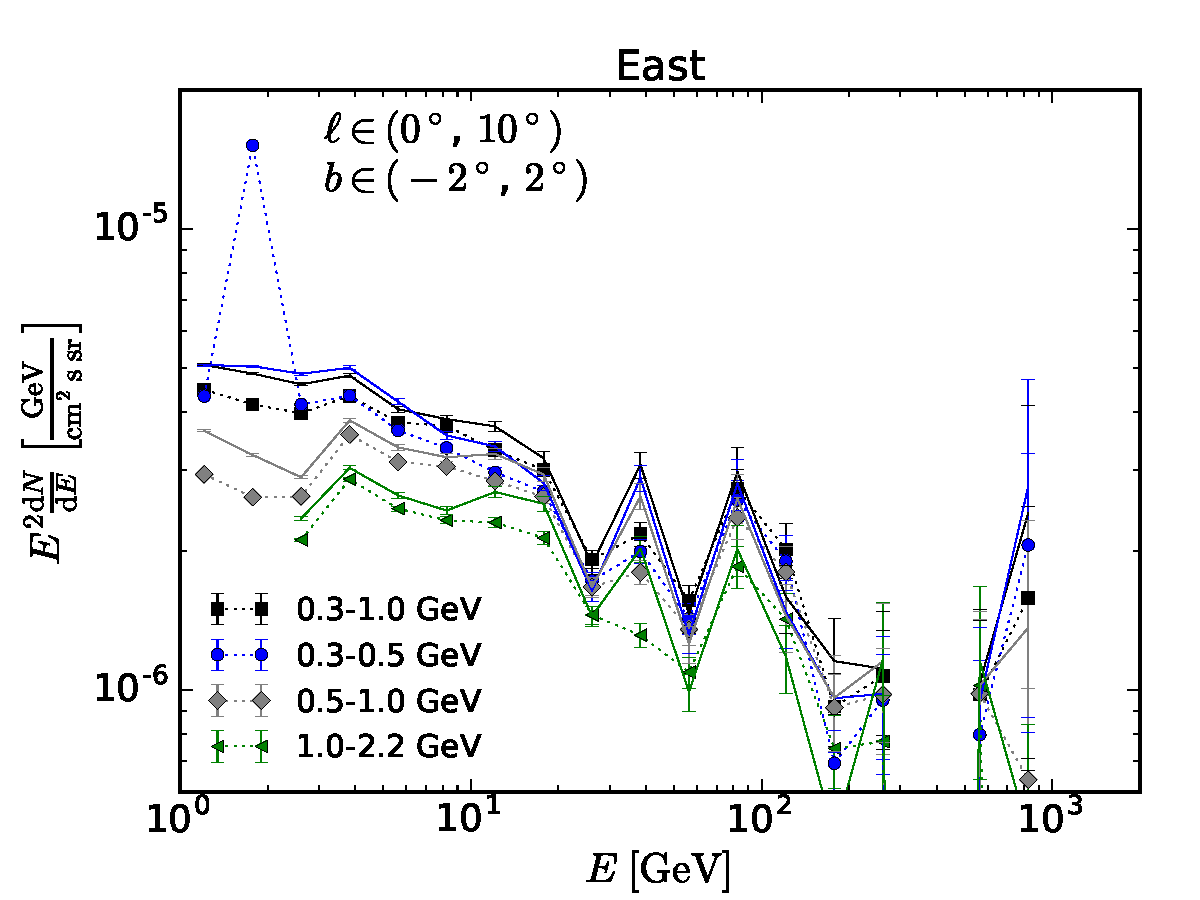
\includegraphics[width=0.5\textwidth]{plots/SED_different_lowE_ranges_boxes_l=5_b=0.pdf}
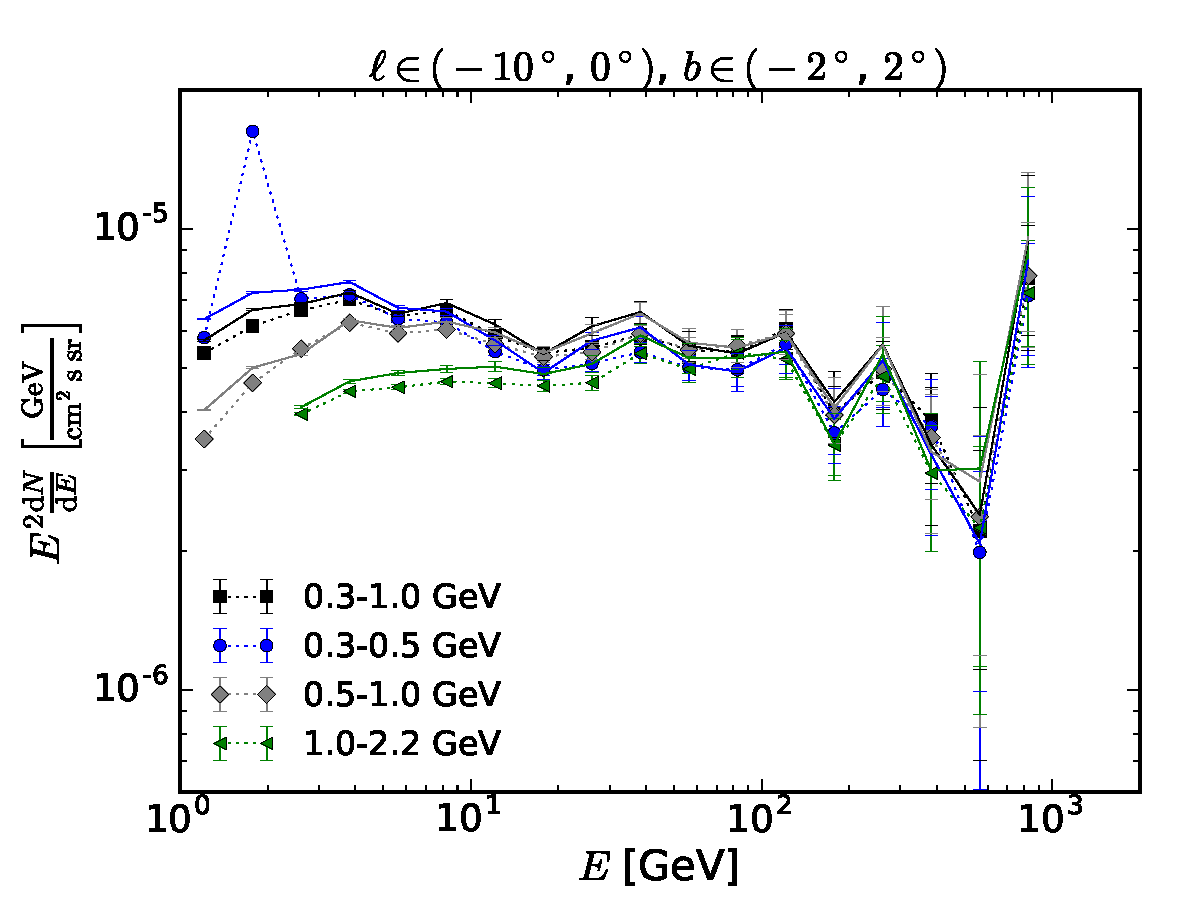
\includegraphics[width=0.5\textwidth]{plots/SED_different_lowE_ranges_boxes_l=-5_b=0.pdf}
  	\caption{SED of rectangles model of source-class (dotted with markers) and ultraclean-class data (solid) in four different energy ranges. $0.3 - \SI{1.0}{GeV}$ (black) is the baseline low-energy range.}
  	\label{fig:syst_models}
\end{figure*}